\section{Autómata celular neuronal en malla}

Niklasson et al. \cite{niklassonMNCA} y Mordvintsev et al. \cite{niklassonMNCA2} \cite{mordvintsevUNCA} introducen el concepto de texturas autoorganizadas, cuyo objetivo es reproducir la apariencia global de una textura de referencia sin generar copias exactas. Para esto, entrenan un autómata celular neuronal utilizando la misma estructura neuronal que se propuso en \cite{mordvintsevNCA}, para que pueda reconocer y crear patrones distintivos como tableros de ajedrez, líneas o mosaicos. Aunque este enfoque tiene un carácter demostrativo, constituye una evidencia significativa de que los autómatas celulares neuronales pueden aprender y generalizar comportamientos visuales locales en lugar de memorizar imágenes específicas.

Niklasson et al. proponen los autómatas celulares neuronales en mallas \cite{meshNCA}, que es un método creado para crear texturas en movimiento en superficies en 3D. A diferencia de los experimentos en cuadrículas de dos dimensiones, los autómatas celulares neuronales en mallas aplican el mecanismo de autoorganización a mallas de cualquier forma, incluso si están en movimiento. El modelo es consistente en diferentes situaciones, es resistente a cambios externos y permite ajustar características como la densidad, la dirección y la rotación de los patrones que aparecen. Además, varios autómatas celulares neuronales en redes pueden combinarse, creando cambios suaves entre texturas sin interrupciones.

\begin{figure}[htbp]
	
	\centering
	
	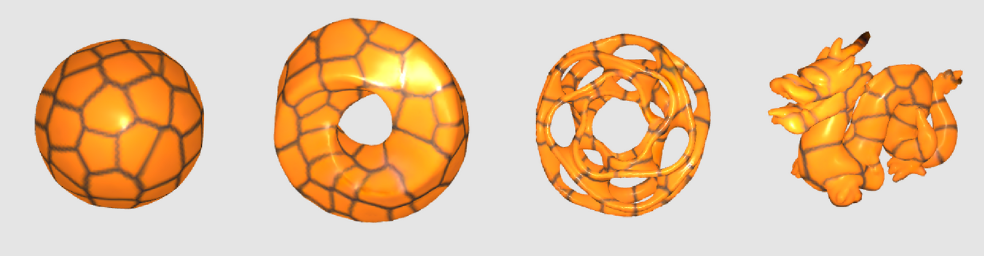
\includegraphics[width=0.75\linewidth]{img/mesh.png}
	
	\caption{El entrenamiento se realiza sobre un poliedro simétrico y el autómata celular neuronal puede ser extrapolado a cualquier objeto tridimensional \cite{mordvintsevNCA}.}
	
	\label{fig:mesh}
	
\end{figure}

Sin embargo, este enfoque presenta un reto de escalabilidad. El número de células involucradas suele encontrarse en el rango de $10^4 \sim 10^5$, lo que limita la resolución alcanzable a entre $64 \times 64$ y $256 \times 256$ píxeles. Como el tiempo de entrenamiento escala de forma cuadrática con respecto al número de celdas, el aumento de resolución conlleva un cuello de botella en la propagación de información a lo largo de la malla.

Para solucionar esta limitación, Niklasson et al. sugieren en \cite{meshNCA2} un modelo híbrido que une autómatas celulares neuronales  con representaciones neuronales implícitas. La idea central es desacoplar el tamaño de la cuadrícula de los autómatas celulares neuronales  de la resolución final, delegando el renderizado detallado a un decodificador ligero denominado red local de producción de patrones. De este modo, el autómata celular neuronal mantiene una cuadrícula explícita y relativamente pequeña que evoluciona de manera local, mientras que la red local de producción de patrones se encarga de producir el color en cualquier punto del espacio continuo a partir de información interpolada de las celdas vecinas.

En términos formales, para cada punto de muestreo $p$, la red local de producción de patrones recibe dos entradas. Una es un estado celular promedio $s(p)$, obtenido mediante interpolación de las celdas cercanas en un primitivo geométrico. La otra es un vector de coordenadas locales $u(p)$, que codifica la posición relativa de $p$ dentro de dicho primitivo. Dependiendo de cómo se divida el espacio, estas formas básicas pueden ser rectángulos, cubos, triángulos o polígonos en general. Estas formas están definidas por coordenadas $\lambda_i(p)$ que deben cumplir con ciertas propiedades, como ser una partición unitaria y no ser negativas. Para asegurar una continuidad en el espacio, se cambian las coordenadas usando funciones sinusoidales en cuadrículas cartesianas o en redes triangulares, creando así campos posicionales suaves.

El resultado es un sistema que conserva las propiedades autoorganizativas de los autómatas celulares neuronales al tiempo que permite alcanzar mayor resolución sin un aumento proporcional del costo computacional. Desde una perspectiva biológica, el autómata celular neuronal puede interpretarse como un plano morfogenético que define la organización global, mientras que la red local de producción de patrones añade los detalles finos sin necesidad de simular interacciones locales a gran escala. Este paralelismo, aunque principalmente ilustrativo, refuerza la idea de que los autómatas celulares neuronales pueden actuar como generadores de estructuras robustas y adaptables, mientras que módulos complementarios aportan precisión y escalabilidad.

A pesar de estas mejoras, una limitación persistente es que cada autómata celular neuronal debe entrenarse de manera específica para una textura o patrón dado. Incluso en escenarios donde múltiples autómatas celulares neuronales coexisten, cada modelo requiere su propio entrenamiento independiente. Esto ha motivado nuevas propuestas orientadas a la construcción de espacios compartidos de autómata celular neuronal, capaces de generalizar a múltiples texturas dentro de un mismo marco de entrenamiento.